\section{1D Burgers Equation Dataset}

%% ---------------------------------------------------------------
%% SLIDE 1: Dataset structure
%% ---------------------------------------------------------------
\begin{frame}{\large Dataset: 1D Burgers Equation Trajectories}
\vspace{-0.5em}
  \begin{columns}[t]
    \begin{column}{0.55\textwidth}
      \begin{block}{\centering \small Where does the data come from?}
        We use the \textbf{official dataset} from the FNO paper
        (Li et al., 2021). The trajectories were generated by
        numerically solving the 1D Burgers equation and saving
        the full solution over time.
        \begin{itemize}\setlength\itemsep{1pt}
          \item \textbf{Domain}: $x \in [0,1]$, $t \in [0,1]$.
          \item \textbf{Periodic boundary conditions}.
          \item Fixed \textbf{viscosity} values: $\nu \in \{0.001, 0.004, 0.01, 0.02, 0.1, 0.3, 0.5, 0.7\}$.
          \item \textbf{1000 train + 200 test} per resolution.
        \end{itemize}
      \end{block}
    \end{column}
    \begin{column}{0.46\textwidth}
      \begin{block}{\centering \small Four grid resolutions}
        \begin{center}
        \small {$85 \times 85$, $141 \times 141$,}\\[0.4em] \small{$211 \times 211$, $421 \times 421$}
        \end{center}
      \end{block}
      \begin{block}{\centering \small Initial conditions}
        \begin{itemize}
            \item The initial condition $u(x,0)$ is randomly generated for each trajectory.
            \item \item From three families:
            \begin{itemize}\setlength\itemsep{1pt}
              \item \textbf{Random Fourier modes:} $u(x,0) = \sum_{n=1}^N A_n \sin(2\pi k_n x + \phi_n)$, with random $A_n$, $k_n$, and $\phi_n$.
              \item \textbf{Single sine waves:} $u(x,0) = A \sin(2\pi k x + \phi)$, with random $A$, $k$, and $\phi$.
              \item \textbf{Two-mode sines:} $u(x,0) = A_1 \sin(2\pi k_1 x + \phi_1) + A_2 \sin(2\pi k_2 x + \phi_2)$, with random parameters.
            \end{itemize}
            \item This variety ensures the model learns to handle a wide range of initial conditions, from simple to complex.
        \end{itemize}
        \end{block}
    \end{column}
  \end{columns}

\end{frame}

%% ---------------------------------------------------------------
%% SLIDE 2: Visualizations - 2x2 grid (s=85 and s=421, nu=0.01 and nu=0.3)
%% Replace each \fbox with \includegraphics[width=\linewidth]{path/to/image.png}
%% ---------------------------------------------------------------
\begin{frame}{Visualizing the Data: 2x2 Grid of Trajectories}

  % Column headers
  \begin{columns}[c]
    \begin{column}{0.02\textwidth}\end{column}
    \begin{column}{0.47\textwidth}
      \centering\small\textbf{$\nu = 0.01$ --- shock}
    \end{column}
    \begin{column}{0.47\textwidth}
      \centering\small\textbf{$\nu = 0.3$ --- smooth}
    \end{column}
  \end{columns}

  \vspace{0.2em}

  % Row 1: s=85
  \begin{columns}[c]
    \begin{column}{0.04\textwidth}
      \rotatebox{90}{\scriptsize\textbf{$s=85$}}
    \end{column}
    \begin{column}{0.46\textwidth}
      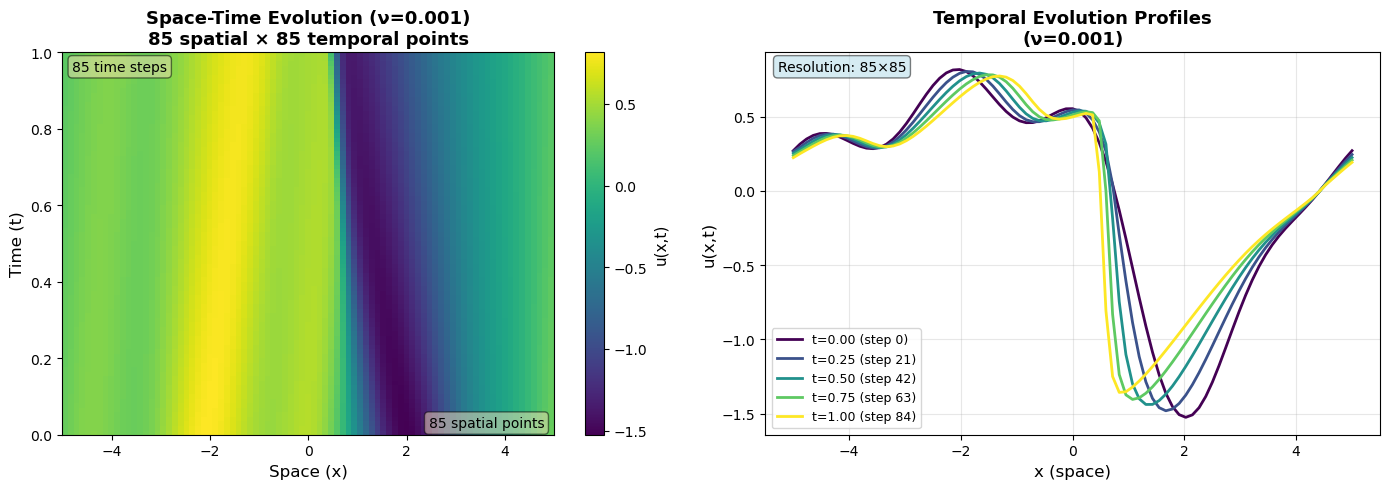
\includegraphics[width=\linewidth, height=2.5cm, keepaspectratio]
        {images/burger/sample_85x85_nu0001.png}
    \end{column}
    \begin{column}{0.46\textwidth}
      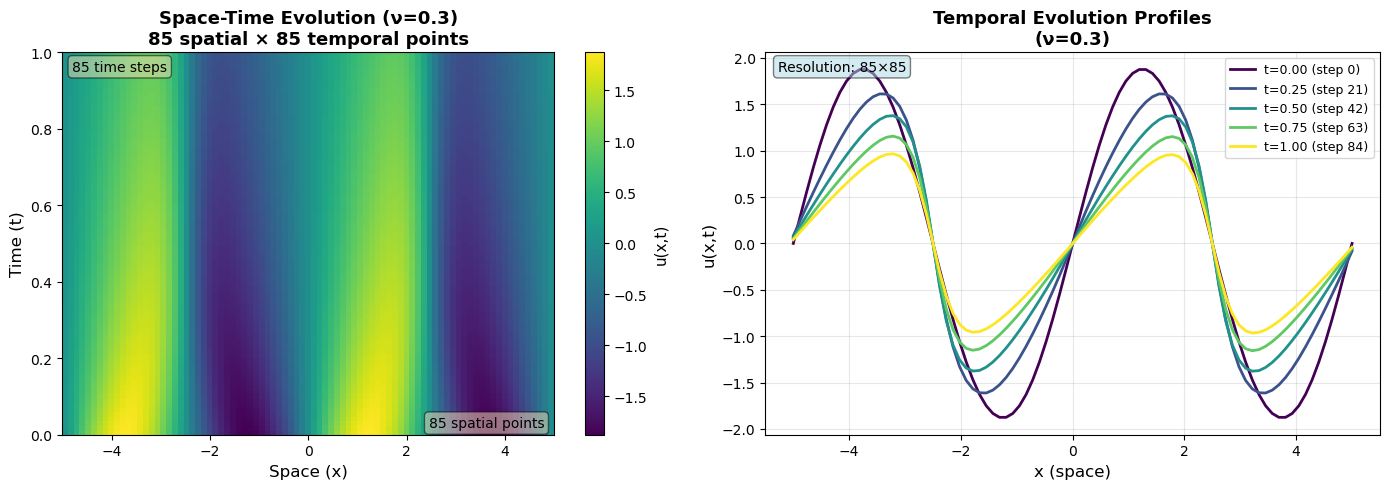
\includegraphics[width=\linewidth, height=2.5cm, keepaspectratio]
        {images/burger/sample_85x85_nu03.png}
    \end{column}
  \end{columns}

  \vspace{0.2em}

  % Row 2: s=421
  \begin{columns}[c]
    \begin{column}{0.04\textwidth}
      \rotatebox{90}{\scriptsize\textbf{$s=421$}}
    \end{column}
    \begin{column}{0.46\textwidth}
      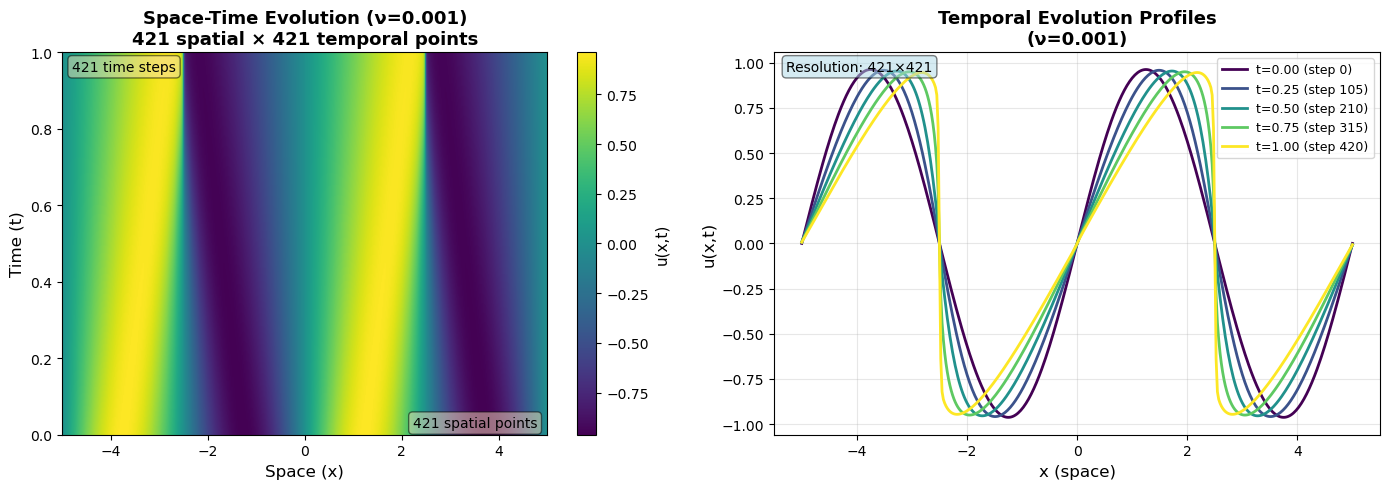
\includegraphics[width=\linewidth, height=2.5cm, keepaspectratio]
        {images/burger/sample_421x421_nu0001.png}
    \end{column}
    \begin{column}{0.46\textwidth}
      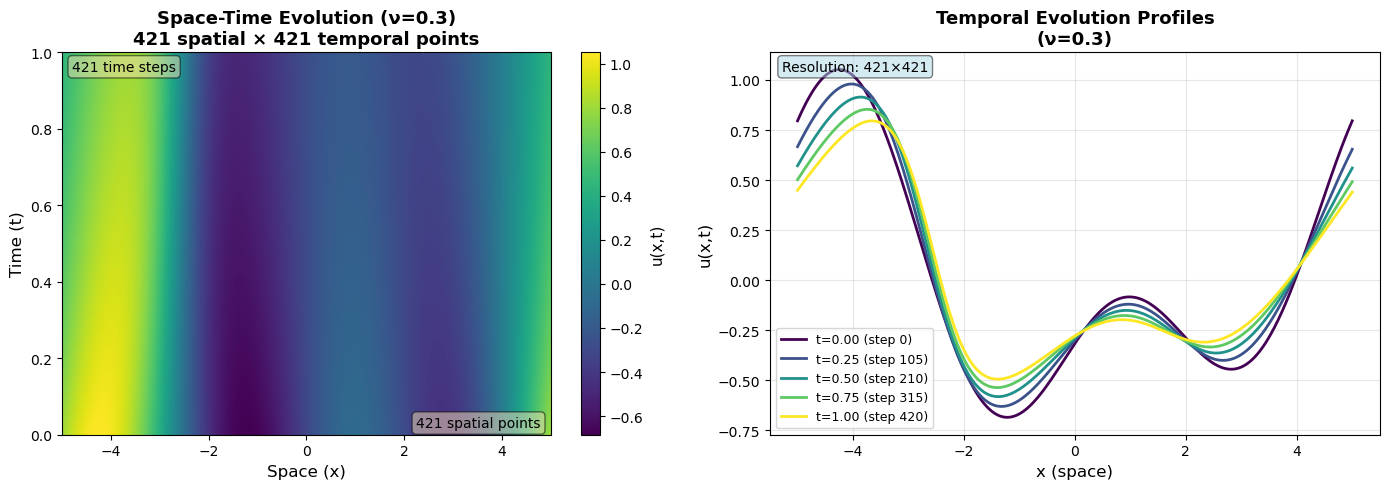
\includegraphics[width=\linewidth, height=2.5cm, keepaspectratio]
        {images/burger/sample_421x421_nu03.png}
    \end{column}
  \end{columns}

  \vspace{0.3em}

  \begin{columns}[t]
    \begin{column}{0.48\textwidth}
      \small Sharp diagonal band = shock moving across the domain.
      Finer grid ($s=421$) captures it more precisely.
    \end{column}
    \begin{column}{0.48\textwidth}
      \small Smooth gradient = diffusion spreading the wave.
      Looks similar at both resolutions --- easy case.
    \end{column}
  \end{columns}

\end{frame}

%% ---------------------------------------------------------------
%% SLIDE 3: Effect of viscosity explained
%% ---------------------------------------------------------------
\begin{frame}{Effect of Viscosity $\nu$}

  \begin{columns}[t]
    \begin{column}{0.48\textwidth}
      \begin{block}{$\nu = 0.01$ --- shock regime}
        \begin{itemize}\setlength\itemsep{2pt}
          \item Advection wins over diffusion
          \item The wave steepens and forms a \textbf{near-shock}
          \item Very sensitive to the initial condition
          \item \textbf{Hard for the model} --- fast changes, sharp features
        \end{itemize}
      \end{block}
    \end{column}
    \begin{column}{0.48\textwidth}
      \begin{block}{$\nu = 0.3$ --- smooth regime}
        \begin{itemize}\setlength\itemsep{2pt}
          \item Diffusion wins over advection
          \item The wave spreads out and flattens
          \item Predictable, regular dynamics
          \item \textbf{Easier for the model} --- slow, smooth changes
        \end{itemize}
      \end{block}
    \end{column}
  \end{columns}

  \vspace{0.4em}

  \begin{center}
  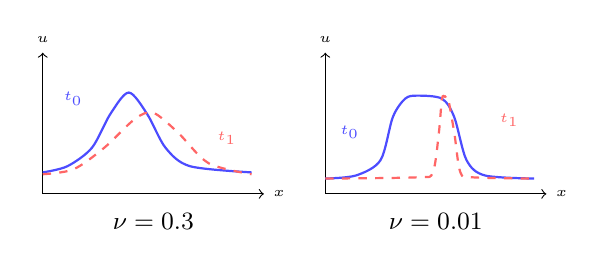
\begin{tikzpicture}[scale=0.78]
    \draw[->] (0,0)--(3.6,0) node[right]{\tiny $x$};
    \draw[->] (0,0)--(0,2.3) node[above]{\tiny $u$};
    \node at (1.8,-0.45) {\small $\nu=0.3$};
    \draw[blue!70, thick] plot[smooth] coordinates {
      (0,0.35)(0.4,0.45)(0.8,0.75)(1.1,1.3)(1.4,1.65)(1.7,1.3)(2.0,0.75)(2.4,0.45)(3.4,0.35)};
    \draw[red!60, dashed, thick] plot[smooth] coordinates {
      (0,0.32)(0.5,0.40)(1.0,0.75)(1.5,1.22)(1.8,1.32)(2.2,1.0)(2.7,0.50)(3.4,0.32)};
    \node[blue!70, font=\tiny] at (0.5,1.55) {$t_0$};
    \node[red!60,  font=\tiny] at (3.0,0.90) {$t_1$};
    \begin{scope}[xshift=4.6cm]
      \draw[->] (0,0)--(3.6,0) node[right]{\tiny $x$};
      \draw[->] (0,0)--(0,2.3) node[above]{\tiny $u$};
      \node at (1.8,-0.45) {\small $\nu=0.01$};
      \draw[blue!70, thick] plot[smooth] coordinates {
        (0,0.25)(0.5,0.30)(0.9,0.55)(1.1,1.25)(1.3,1.55)(1.5,1.60)(1.9,1.55)(2.1,1.25)(2.3,0.55)(2.6,0.30)(3.4,0.25)};
      \draw[red!60, dashed, thick] plot[smooth] coordinates {
        (0,0.25)(1.5,0.27)(1.75,0.35)(1.85,1.0)(1.90,1.55)(1.95,1.58)(2.0,1.55)(2.1,1.0)(2.2,0.35)(2.4,0.27)(3.4,0.25)};
      \node[blue!70, font=\tiny] at (0.4,1.0) {$t_0$};
      \node[red!60,  font=\tiny] at (3.0,1.2) {$t_1$};
    \end{scope}
  \end{tikzpicture}
  \end{center}

\end{frame}

%% ---------------------------------------------------------------
%% SLIDE 4: Multi-resolution evaluation
%% ---------------------------------------------------------------
\begin{frame}{Testing at 4 Different Resolutions}

  \begin{block}{Why do we test at 4 resolutions?}
    We want to know if our model works well regardless of how fine the
    grid is. A good model should give similar accuracy at $s=85$ and
    at $s=421$ --- this is called \textbf{resolution consistency}.
    We trained one TCAN model per resolution, all with the same
    architecture, and compared the results.
  \end{block}

  \vspace{0.4em}

  \begin{columns}[t]
    \begin{column}{0.48\textwidth}
      \begin{block}{What changes with resolution?}
        \begin{itemize}\setlength\itemsep{2pt}
          \item Finer grid $\Rightarrow$ more spatial points
          \item More time steps $\Rightarrow$ longer rollout
          \item Longer rollout $\Rightarrow$ more accumulated error
          \item So higher $s$ is naturally harder for TCAN
        \end{itemize}
      \end{block}
    \end{column}
    \begin{column}{0.48\textwidth}
      \begin{block}{Viscosity regimes in the data}
        \begin{center}
        \small
        \begin{tabular}{ll}
          \toprule
          $\nu$ range & Behaviour \\
          \midrule
          $(0,\,0.05)$   & Near-shock \\
          $(0.05,\,0.3)$ & Transitional \\
          $(0.3,\,1.0)$  & Smooth \\
          \bottomrule
        \end{tabular}
        \end{center}
        Since $\nu \sim \mathcal{U}(0,1)$, all three regimes
        appear in both train and test sets.
      \end{block}
    \end{column}
  \end{columns}

\end{frame}